\documentclass{article}

\usepackage[utf8]{inputenc}
\usepackage{graphicx}

\title{Rapport de projet web}
\author{Alexandre Garand, Lucas Bourel, Corentin Guillerme, Maxime Song}

\begin{document}

\maketitle
\newpage

\section{L'architecture}
	Nous avons choisit d'utiliser une structure modèle-vue-contrôleur.\\ \\
	Nous avons un fichier index.php qui est un routeur dirigeant vers toutes les pages du sites et est le seuls point d’accès de ces pages.\\ \\
	Ensuite nous avons un fichier template.php qui donne la structure de toutes les pages du sites contenant notamment l'en tète et le pied de la page.\\ \\
	Ensuite pour chaque page nous avons un fichier de vue contenant le contenue spécifique de la page.\\ \\
	Pour chaque page non-statique nous avons un fichier contrôleur qui décide quoi afficher pour ces pages en fonction du contexte.\\ \\
	Pour chaque table de la base de donnée nous avons un fichier avec une classe représentant la table avec les mêmes attributs et des accesseur et mutateurs pour modifier la classe et un fichier manager manipulant la base de donnée et la classe php pour permettre d'accéder et traiter les données.\\ \\
	Le principe du site web est donc d'avoir index.php qui appelle le contrôleur de la page web à afficher, le contrôleur peut utiliser les classes du modèle pour manipuler la base de donnée puis il envoie la vue de la page à afficher à template.php qui affiche la page.
\section{Le modèle}
	\subsection{Les bases de données}
		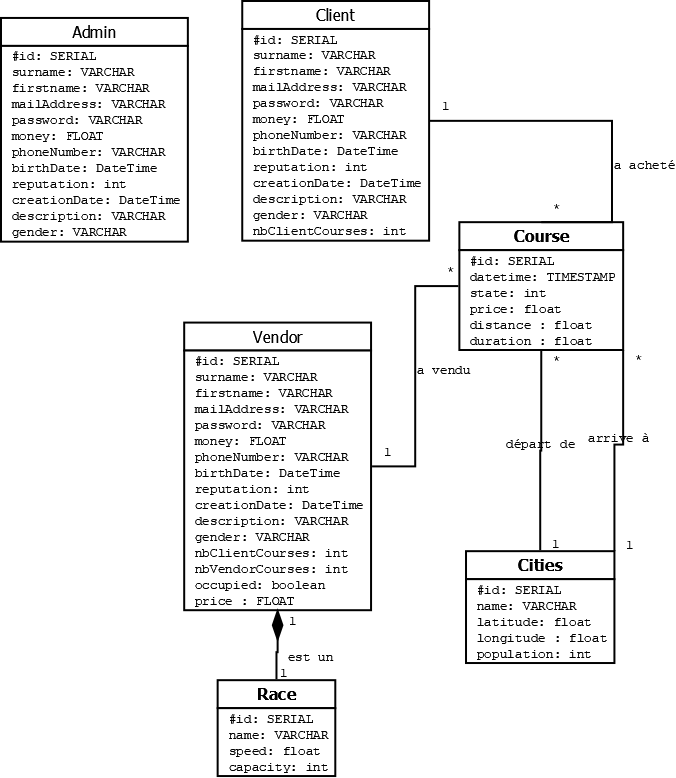
\includegraphics[scale=0.3]{diagrammeTotal.png} \\
		\subsubsection{Admin/Client/Vendor}
			Ces trois tables représentent les utilisateurs selon leur rôle et contient toutes les informations afin de permettre l'utilisation du sites ainsi que des informations classiques sur les utilisateurs. Il est important de noter que le vendeur est peut aussi utiliser le site en tant que client.
		\subsubsection{Race}
			Cette table contient le nom et les caractéristique de la race afin de savoir comment les clients serons servis par la race en question.
		\subsubsection{Course}
			Celle-ci contient les informations sur les transports effectués afin de permettre aux utilisateurs d'accédés à l'historique de leurs transactions.
		\subsubsection{Cities}
			Celle-ci contient les informations sur les villes: les coordonnées gps pour pouvoir les placés et la population pour pouvoir les trier dans la liste des propositions pour l’auto-complétion.
	\subsection{Le programme}
		\subsubsection{Principe général}
			Pour chacune des tables de la base de donnée afin de pouvoir les manipuler efficacement en php chaque table est représenter par une classe possédant les mêmes attributs que la bases de donnée, un accesseur pour chaque attribut et un mutateur pour chaque sauf ceux qui ne doivent pas être modifier tels que l'id ou la date de création d'un compte.
		\subsubsection{Cas particulier de User}
			Une classe de plus à été ajouter au modèle: la classe User.\\ Celle-ci est la classe mère de Admin Client et Vendor permettant de ne pas avoir à réécrire la même chose trois fois pour chaque attribut en commun pour les trois.
		\subsubsection{Les managers}
			Les managers permettent de lire la base de donnée et de convertir une ligne de la table en une instance de la classe correspondant et vis-versa : elle permet d'ajouter, de détruire, de modifier ou d'accéder à une ligne de la base de donnée ou d'accéder à toutes les lignes. Il y à aussi des opérations spécifiques à certaines tables comme dans Cities qui à une fonction spécifique pour l'auto-complétion allant chercher les villes commençant par une chaîne de caractère.
	\subsection{Problèmes rencontrés et solutions}
		\subsubsection{Les injections SQL}
			Un problème que nous avons eu est la possibilité d'effectué des injections SQL en effet avec la fonction query l'utilisateur pouvait utiliser la chaîne de caractère qu'il voulait pour faire faire ce qu'il voulait à la base de donnée.\\ Pour palier à ce problème nous avons utiliser la fonction prepare qui empêche ce genre d'acte malveillant.
		\subsubsection{Les injections SQL}
			Le deuxième problème rencontrer est l'héritage de User qui n'a pas pus être fais au niveau de la base de donnée ce qui à été pallié en écrivant trois base de donnée distincte avec des données similaires. Cette solution peu efficace à causer une duplication du code importante et un héritage peu utile au niveau des managers.
			
\section{Le contrôle}
\section{La vue}
\section{La répartition}

\end{document}